\subsection{$\Zo$ boson selection\label{sec:Z}}
\par
To identify $\Zll$ decays,
a pair of identified leptons is required, with dilepton invariant
mass in the range $60 < \MLL < 120\GeV$.
Backgrounds are very low, including backgrounds from QCD processes.
In the $\Zee$ channel, the yield is obtained by counting the number
of selected events and making a small correction for backgrounds.
In the $\Zmm$ channel,
yield and lepton efficiencies are fitted simultaneously.
No correction is made for $\gamma^*$ exchange.

\subsection{$\Zee$ signal extraction\label{sec:Zee}}
\par
The $\Zee$ candidate events are required to have two electrons satisfying
the same selection criteria as the electrons selected
in the $\Wen$ sample.  Both electrons must have an ECAL cluster with
$\et > 25$~GeV in the ECAL fiducial volume.
%The fraction of signal events selected in the simulation is
%$\APRIM{Z}=\ZEEAPRIM$.
\par
The $\Zo$ mass peaks in the data exhibit small shifts 
%%, on the order of 1 to 2\%,
with respect to the simulated distributions.
From these shifts, we determine
ECAL cluster energy
scale correction factors 
%of \EBESCALE and \EEESCALE
for barrel and endcap electrons, respectively.
The uncertainties on these correction factors are
propagated as systematic uncertainties on the yield.
Applying these corrections to
electron candidates in the data, we
select $\ZEESAMPLEN$ events, with the dielectron invariant mass
shown in Fig.~\ref{fig:Zee}~(a),
along with the predicted distribution,
after the energy scale correction of the data and normalization of the
simulation.

%%%%%
\begin{figure}
  \begin{center}
   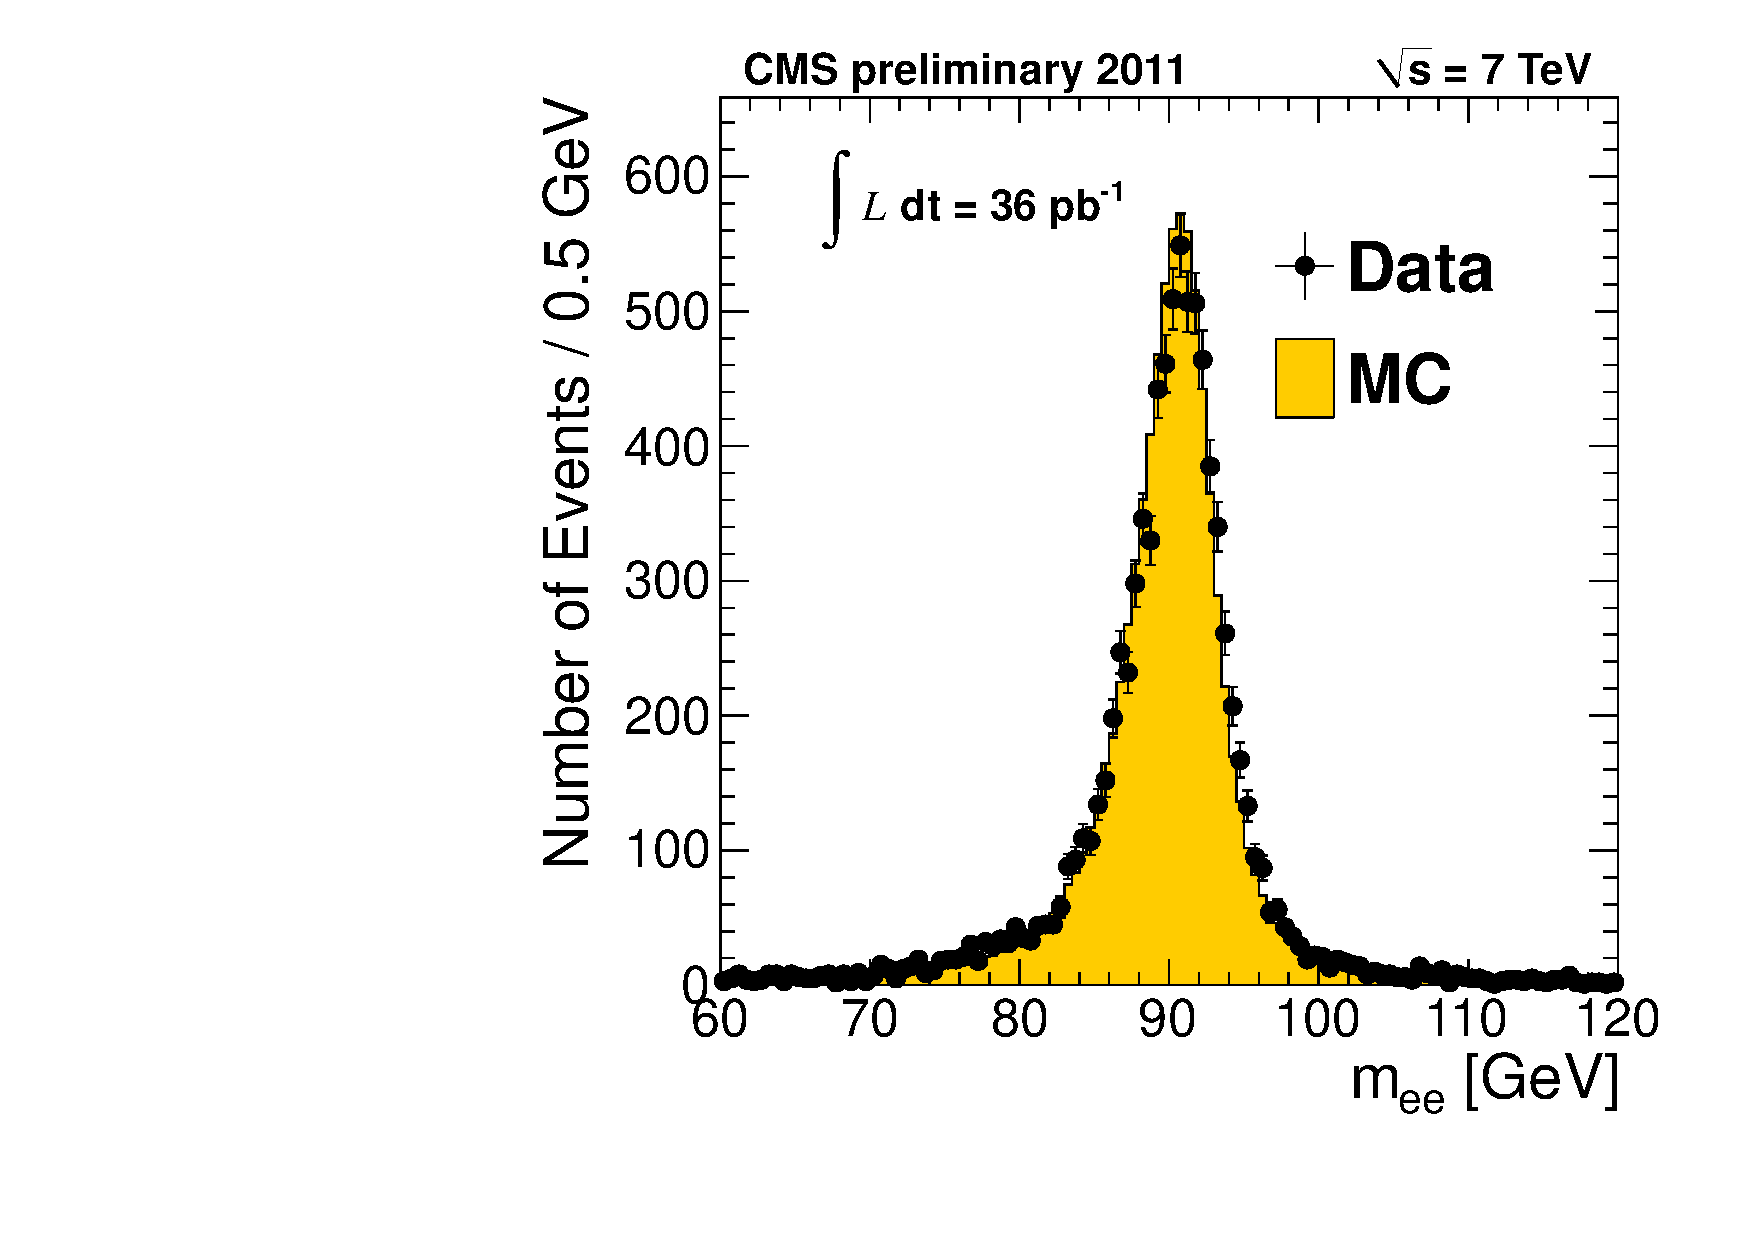
\includegraphics[width=0.48\textwidth]{figs/Zee_mass_Linear.pdf}
   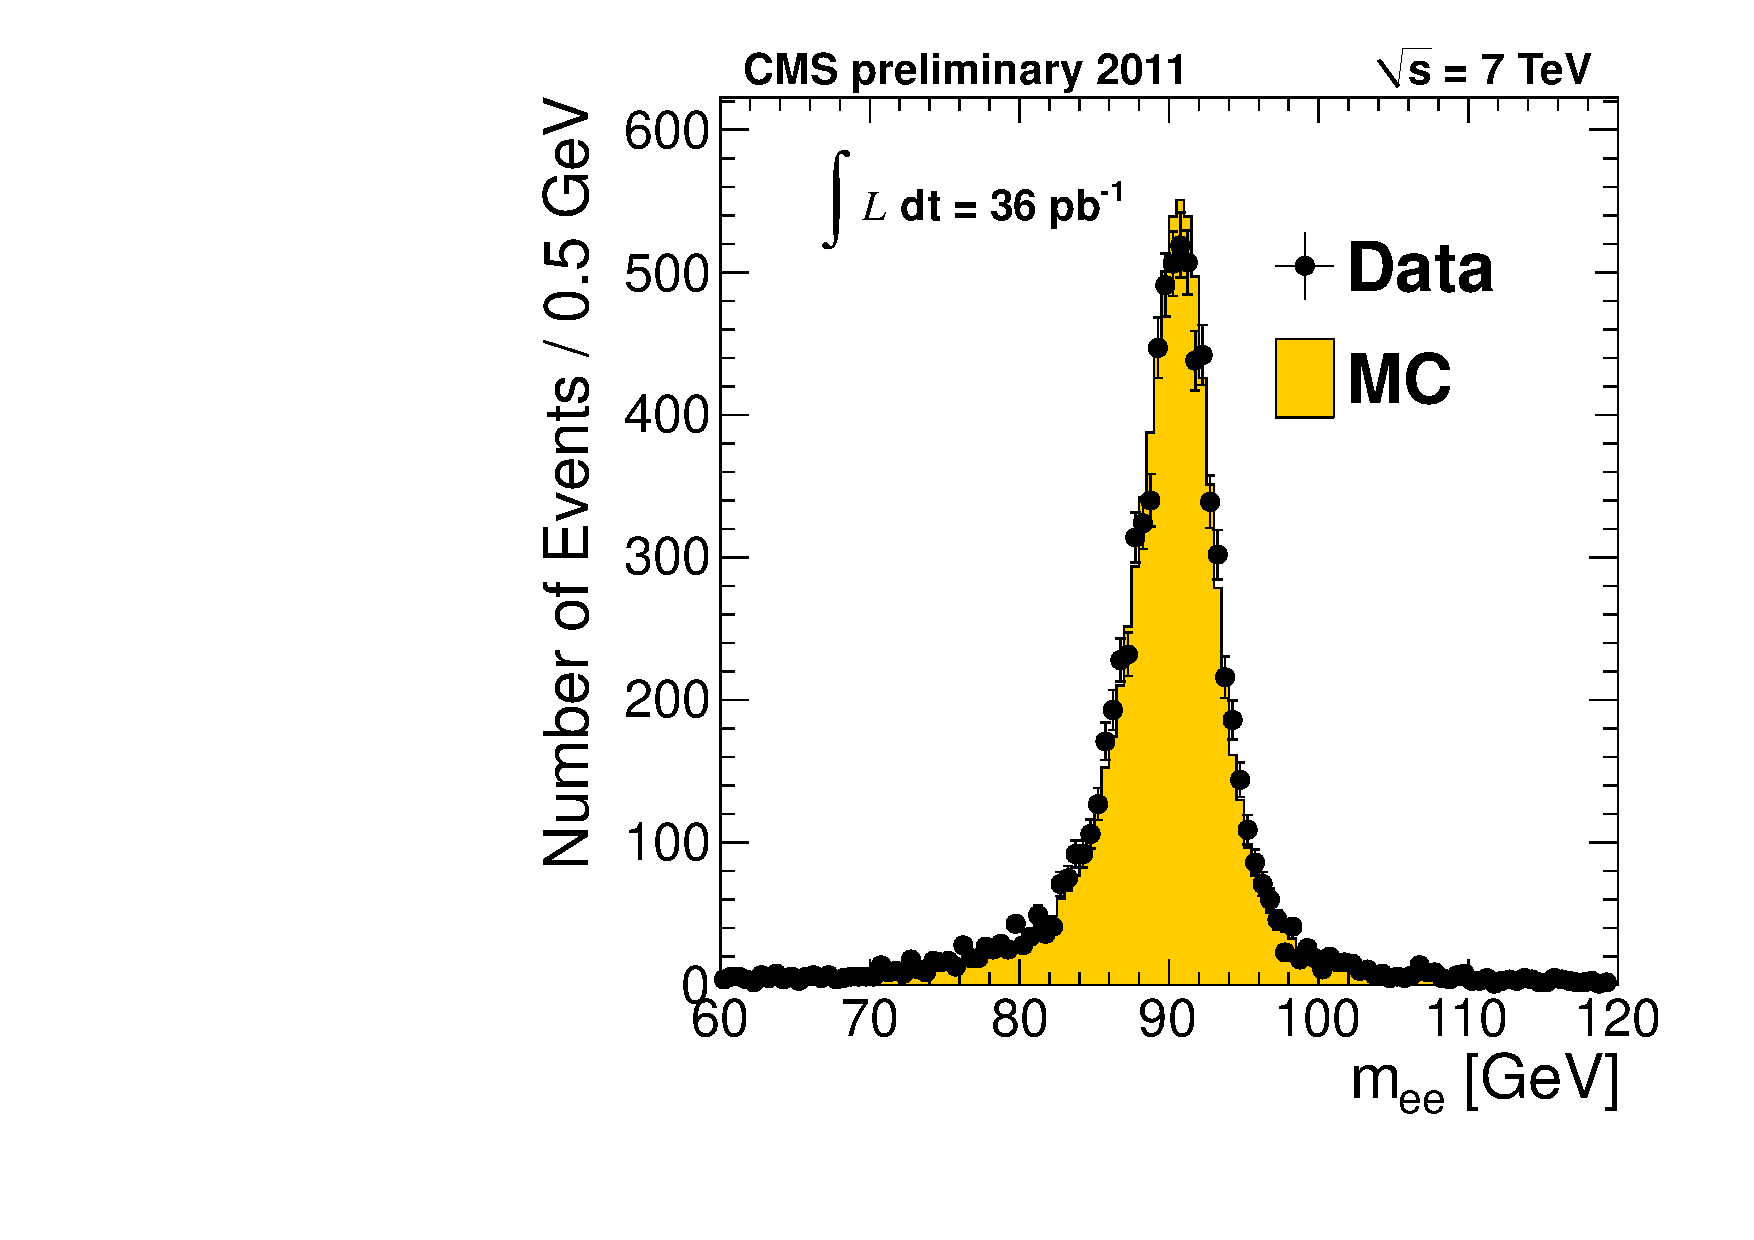
\includegraphics[width=0.48\textwidth]{figs/Zee_mass_Linear_corrected.pdf}
   \caption{ \label{fig:Zee}
$\Zee$ signal in linear scale before (left) and after applying energy scale correction
factors (right). The points represent the data, and the histograms, the expected
distribution from simulations normalized to $36$~pb$^{-1}$
and NNLO cross sections.  Backgrounds are negligible and
cannot be seen on the linear scale plot. Plots obtained with the WP80
electron selection.  }
  \end{center}
\end{figure}
%%%%%



\par
Two techniques are used to estimate the background originating from events in which
one or both electron candidates are misidentified jets or photons.
The first method uses a fit to the track isolation variable to extract the
fractions of signal and QCD background. The second method is based on counting 
events with electron candidates of same electric charge, after taking into account 
the probability of wrong charge assignment. 
The two methods are independent and give consistent results.
we will use the estimation of the first method in the analysis since it is much more
accurate. The second method will serve as a cross check.
We estimate the QCD background in our sample to 
be $\ZEEQCDBKG$ events. Backgrounds from other processes with true 
electrons ($\Ztt$, dibosons, and $\ttbar$) are estimated from the simulation. 
The total background in the $\Zee$ sample is estimated to be \ZEEBKG events.
